% Built by Seshat-Star/analysis/method_fig.py (11-17, v8): scene0406_00, ScanRefer val item scene0406_00_ann1_obj21, towel #21 of 8.
% The rewrite, the reader's five predicates and the five surviving sets are the stored outputs for this item (re-evaluated 11-17:
% 1 / 3 / 1 / 3 / 5 towels, intersection {21}, strict).  The evidence chips carry facts from this item's real fact block (ids and
% numbers as computed, wording shortened); their colours pair each with the clause stating the same relation - matched by content,
% the system does not record which fact the writer used.  The writer's view is redrawn for print from the same point cloud and
% masks (one camera, cropped; anchors take their clause's colour).  Label font: Comic Neue (SIL OFL).
% Canvas 10 x 6.46 in, printed at 6.875 in (4.44 in tall): smallest type 8 pt -> 5.5 pt on the page (tags on the render).
\begin{figure*}[t]
\centering
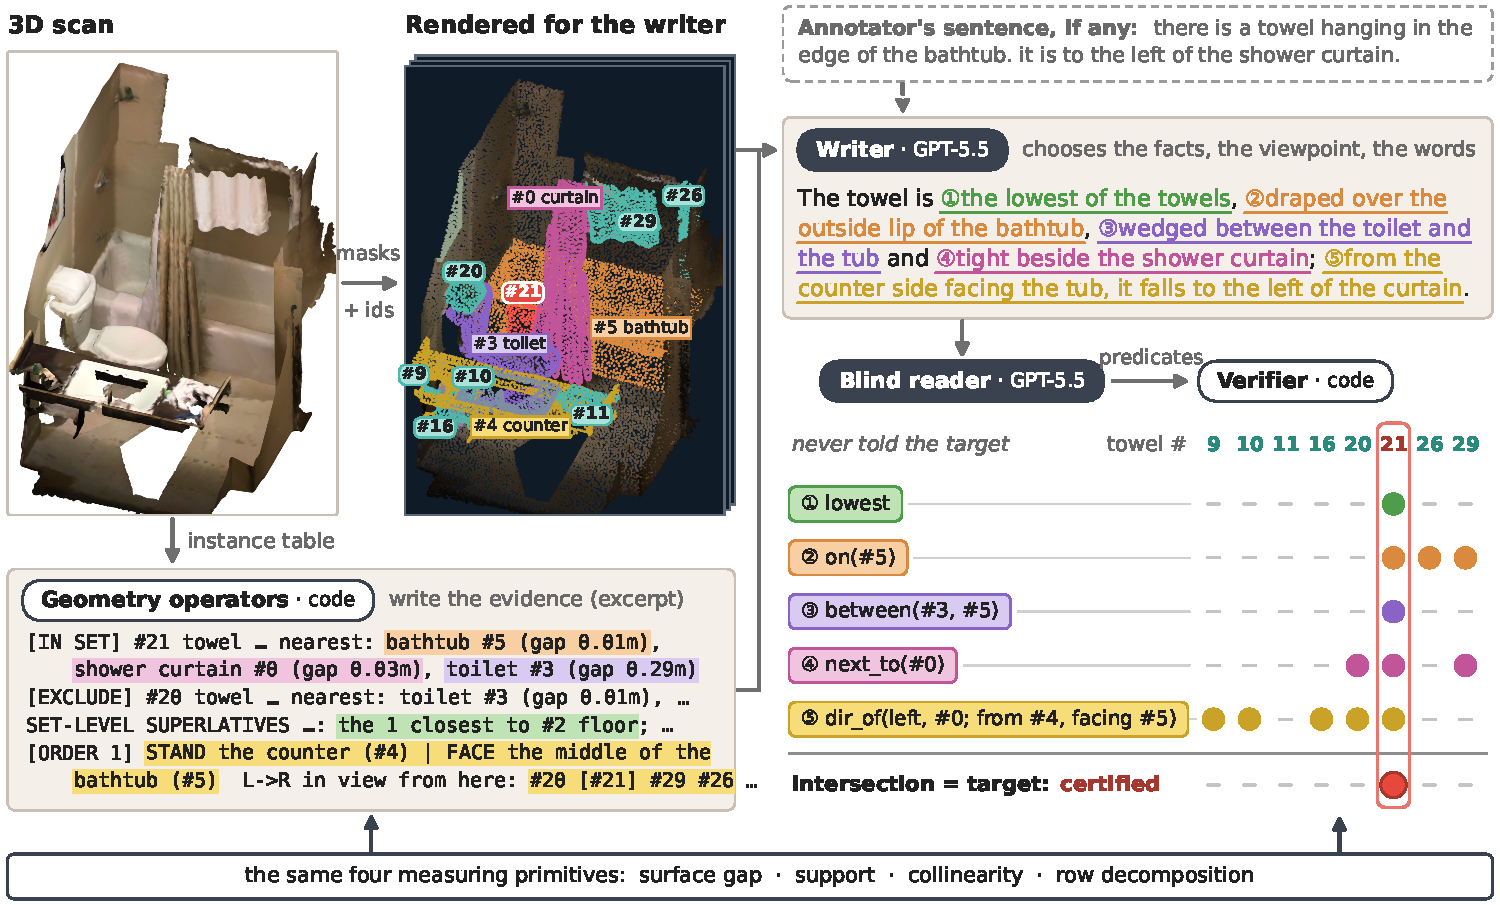
\includegraphics[width=\linewidth]{fig/method.pdf}
\caption{\textbf{One sentence through the four roles}: towel \#21 among eight (ScanRefer val).
Operators compute the evidence, the writer composes the sentence, the blind reader returns one predicate per numbered clause, and the verifier marks the towels each predicate keeps.
The sentence, the predicates and the surviving sets are the stored outputs for this item; the evidence is an excerpt.
No verdict returns to the writer.}
\label{fig:\currfilebase}
\end{figure*}
